\documentclass{report}

% Pacotes para acentuação e formatação

\usepackage[utf8]{inputenc}
\usepackage[T1]{fontenc}
\usepackage[brazil]{babel}
\usepackage{setspace}    % Para espaçamento
\usepackage{lipsum}      % Texto de exemplo (remova se não precisar)
\usepackage{graphicx}




\begin{document}
	
	\begin{titlepage}
	\centering
	\vspace*{5cm} % Espaço do topo
	
	{\Huge\bfseries Arquitetura de Computadores I (LAB)\par} % Título
	
	\vspace{0.5cm}
	{\Large 2025/2\par} % Ano
	
	\vfill
	{\large Nicolas Ramos Carreira\par} % Nome
	
	\vspace*{2cm}
	\end{titlepage}
	
	\tableofcontents
	\newpage
	
	\chapter{Intuito}
	O intuito deste documento é explicar sobre o que será feito nas aulas de laboratório da disciplina de Arquitetura de Computadores I. Neste documento provavelmente estarão explicações de componentes elétricos e alguns conceitos físicos, então se prepare!
	\chapter{Fundamentos Fisicos da Computação}
	\section{Carga elétrica}
	\begin{itemize}
		\item A carga elétrica faz com que a matéria experimente uma força de atração ou repulsão
		\item A medida da carga elétrica é Coulombs (C)
		\item Para fazer uma analogia, podemos dizer que a a carga elétrica seria a água
	\end{itemize}
	\section{Corrente elétrica}
	\begin{itemize}
		\item A corrente elétrica é o movimento da carga elétrica (ou seja, representa uma taxa que mede a intensidade do fluxo elétrico)
		\item A medida da corrente elétrica é feita em Amperes (A)
		\item Em equações, costuma-se utilizar: $1A = 1 C/s$ (1 Amper = 1 Coulumb/segundo)
		\item Para fazer uma analogia, podemos dizer que a corrente elétrica seria: FLUXO DA ÁGUA EM UM PONTO/segundo
	\end{itemize}
	\section{Tensão(voltagem)}
	\begin{itemize}
		\item A tensão influencia a taxa com a qual uma carga flui através de um circuito. É a diferença de potencial elétrico entre dois pontos. Só iremos ter corrente elétrica se houver diferença de potencial.
		\item A tensão é medida em Volts (V)
		\item Para fazer uma analogia, Imagine uma fonte de energia (uma BOMBA D’ÁGUA).Essa bomba aumenta a PRESSÃO DA ÁGUA e aumenta a
		velocidade do fluxo. Essa pressão é a TENSÃO
	\end{itemize}
	\section{Resistência}
	\begin{itemize}
		\item É uma medida da dificuldade da corrente de fluir por um condutor
		\item É medida em Ohms (Ω)
		\item Uma analogia possível seria comparar com o diâmetro do cano
	\end{itemize}
	\section{Analogia(para um entendimento claro)}
	\begin{figure}[ht]
		\centering
		% ajusta a largura da imagem para ser quadrada (ex: 5cm x 5cm)
		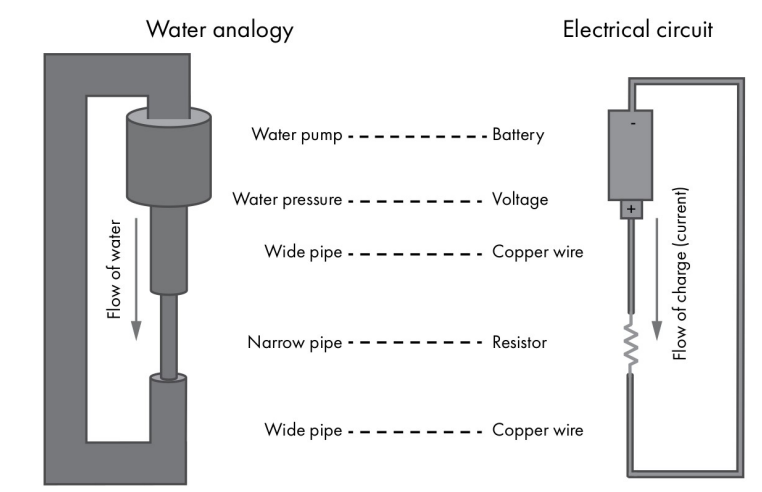
\includegraphics[width=7cm,height=5cm,keepaspectratio=false]{imagens/analogia.png}
		\caption{Water pump = Bomba d'água; Narrow pipe = tubo estreito}
	\end{figure}
	\section{Lei de Ohm}
	\begin{itemize}
		\item A lei de Ohm vai nos dizer que a corrente que flui entre dois pontos é igual à voltagem dividida pela resistência: I = V/R
		\item Seguindo com a analogia, se você aumentar a pressão da água (V), a quantidade de água que flui (I) também aumenta, desde que o entupimento (R) continue o mesmo. Por outro lado, Se o entupimento (R) for maior, a quantidade de água que flui (I) diminui, mesmo que a pressão (V) continue a mesma.
		\item CUIDADO AC X DC: A DC representa a corrente continua, que é quando A corrente flui em apenas uma direção. A maioria das pilhas e baterias usa corrente contínua (guarde esta informação). Por outro lado, temos a AC que representa a corrente alternada, onde os polos se invertem várias vezes para que a corrente continue circulando. A energia que chega nas tomadas das nossas casas é AC. É importante ter cuidado com isso pois no laboratório, durante as atividades, utilizaremos componentes que utilizam a CORRENTE CONTINUA, então não inverta o polo do capacitor na hora de encaixá-lo, pois como vimos, na corrente continua os polos não se invertem.
	\end{itemize}
	\section{Circuitos elétricos (conceitos básicos)}
	\begin{itemize}
		\item É um conjunto de vários componentes (veremos sobre esses componentes mais afrente) conectados de forma a permitir que a corrente possa fluir em um loop, a partir da fonte de energia, passando pelos elementos do circuito, e de volta à fonte de energia
		\item  Um circuito começa e termina no mesmo lugar.
		\item Em circuitos DC, o terra (GND) é considerado 0V e serve como um ponto de referência. Pode ser a terra propriamente dita, ou o polo negativo de uma bateria, por exemplo.
	\end{itemize}
	\section{Lei de Kirchhoff}
	\begin{itemize}
		\item A soma das voltagens em um circuito é 0
		\item Isso significa que se uma bateria fornece 9V para um circuito, os vários componentes do circuito devem “consumir” esses 9V. No caso da imagem abaixo, os resistores fazem esse papel
		
	\end{itemize}
	
	\begin{figure}[ht]
		\centering
		% ajusta a largura da imagem para ser quadrada (ex: 5cm x 5cm)
		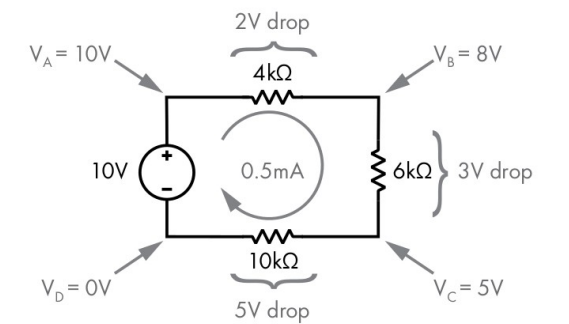
\includegraphics[width=8cm,height=5cm,keepaspectratio=false]{imagens/kirchhoff.png}

	\end{figure}
	
	Acima, os resistores irão consumir a voltagem durante o circuito, até que seja 0V. Mas afinal, como 4kΩ vira 2V, por exemplo? Para isso, usamos a fórmula V = I X R (proveniente da fórmula I = V/R). Assim teremos que:
	\begin{itemize}
		\item Corrente (I): O circuito tem uma corrente de 0.5 mA (0.0005 Amperes). corrente é a mesma em todos os resistores nesse tipo de circuito.
		\item Resistência (R): A resistência do resistor em questão é de 4k Ohms (4.000 Ohms).
	\end{itemize}
	
	Com isso, bastará fazer: V = (0.0005 A)×(4000 Ohms), que será igual a 2V. Assim, faremos isso com todos os resistores, resultando em: 2V (o primeiro que fizemos), 3V e 5V. Ao somar a voltagem de todos eles, teremos 10V. Ou seja, os resistores irão consumir a voltagem por completo, atendendo a Lei de Kirchhoff.
	
	Um detalhe é que se tivermos um circuito onde queremos descobrir qual resistor temos que colocar para que ele consuma nossa voltagem, nós usamos a fórmula R = V/I, onde vamos substituir em V quantos volts queremos que esse resistor "gaste". Em I, teremos a corrente que vai passar por esse resistor. Em circuitos simples em série, a corrente é a mesma em todos os componentes. 
	
	\chapter{Cicuito real}
	\section{O que é Arduíno?}
	Arduino é uma plataforma para auxiliar com projetos de eletronica e programação. A ideia é que você tivesse uma coisa barata, funcional (que desse para instalar coisas de verdade) e que fosse fácil de aprender. Essa plataforma é quase todo baseado em uma plaquinha. Veja a foto abaixo:
	
	\begin{figure}[ht]
		\centering
		% ajusta a largura da imagem para ser quadrada (ex: 5cm x 5cm)
		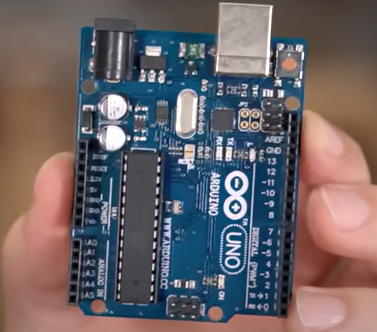
\includegraphics[width=8cm,height=5cm,keepaspectratio=false]{imagens/arduino.png}
		
		\caption{Arduino UNO R3}
		
	\end{figure}
	
	Essa plaquinha tem microcontroladores (a parte preta larga da placa que fica quase no meio) que funciona mais ou menos como um computadorzinho bem pequeno que é capaz de processar e armazenar coisas e também tem uma linguagem de programação, onde você consegue escrever coisas, criar sisteminhas que você coloca dentro e faz com que a placa te obedeça.
	
	E por que o arduino deu tão certo? Pois foi criado com a ideia de hardware livre. Qualquer um pode olhar como funciona seu circuito, comprar os componentes, montar seu próprio arduino e se quiser até vender seu próprio arduino. Isso faz com que o arduino seja barato, sendo assim usado amplamente em projetos, o que contribui para a disponibilização de vários materiais de arduino e com que várias pessoas possam ter contato com ele.
	
	Uma observação é que se pode utilizar o arduíno pela internet a partir do site TinkerCad. Se você comprar a placa, você precisa conectar ela via USB ao computador e baixar o softwere Arduino IDE, onde você bota o código que você vai fazer para enviar para a placa.
	
	Se você quiser ligar a placa sem o computador (isso acontece depois que você ja colocou o programa que voc~e fez nela), você conecta um adptador de bateria de 9V na placa por meio da entrada redonda e conecta o adaptador a bateria, aí você consegue ligar ela assim.
	
	
	
	\section{Principais componentes eletrônicos e ferramentas}
	\section{Circuitos básicos (para entendimento)}

\end{document}